\subsection{\texorpdfstring{Fake background estimation in $\leptonTau$ channel}{Fake background estimation in lepton-tau channel}}
\label{sect:bkgFake}
%{\bf FIXME: numbers and plots should be corrected after applying the tauMT}
In the $e/\mu\Tau$ channels, the main background is the \wjets, when the \Wpm boson decays to a lepton and a jet fakes a hadronic $\tau$.
We use a fake rate method to estimate this background \cite{CMS_AN_2010-261} in the \leptonTau channel.
The idea is that when the loose signal selection is applied, the number of the loose \Tau's ($L$) is:
\begin{equation}
L = P + F
\end{equation}
where $P$ is the number of the  prompt \Tau's and $F$ is the number of the  fake \Tau's. If the selection is tightened, the number of the tight \Tau's (T) is
\begin{equation}
 T = pP + fF
\end{equation} 
$p$ ($f$) is the prompt (fake) rate, the probability that a loosely selected prompt (fake) \Tau can pass the  tight  selection. 
%The loose category ($L$) can be divided to two parts, 
%tight ($T$) and non-tight ($NT$), so one can write:
Solving the system of two equations gives:
\begin{equation}
   F * (f - p) = (T - pL)
\label{eq:F}
\end{equation}
Here, $f$ * $F$ is the contamination of the fake \Tau's in the signal region. 

The fake rate ($f$) is measured as the ratio of the tightly selected \Tau's to the loosely 
selected \Tau's in a data sample which is dominated by the fake \Tau's. The fake rate is estimated in an environment which is as 
similar as possible to the signal region. 
%The dataset and the triggers which are used to estimate the fake rate %in different channels 
%are shown in table \ref{Tab.DataFR}.
%\begin{table}[!htb]
%\begin{center}
%\begin{tabular}{|l|c|c|}
%\hline
%\hline
%Channel      & Data Set                                     & Trigger \\\hline\hline
%Muon Tau     & /SingleMu/Run2012D-22Jan2013-v1/AOD          & HLT\_IsoMu24\_v(16-17)\\
%             &                                              & HLT\_IsoMu24\_eta2p1\_v(14-15)\\\hline
%Electron Tau & /SingleElectron/Run2012D-22Jan2013-v1/AOD    & HLT\_Ele27\_WP80\_v11\\
%\hline
%\end{tabular}
%\caption{The dataset and triggers for fake rate estimation.}
%\label{Tab.DataFR}
%\end{center}
%\end{table}
%In the muTau channel, exactly one muon is required which passes the selection criteria of the muon in the signal region and has \pt > 27 GeV. 
%Lepton selection and extra lepton rejections are exactly same as the signal selection. Only the \pt of the %favorite 
%leading lepton is forced to 
%be 3 \GeV higher than the online cut resulting to \pt $>$ 27 \GeV for muon.% and \pt $>$ 30 \GeV for electron.
%The rejections can reduce the contribution of the VV, DY and $\ttbar$ events. To further suppress the $\ttbar$ contamination, the b-veto 
%similar to the signal selection is applied. The \MPT is asked to be greater than 30 GeV, similar to the preselections. 
All preselection cuts are applied exactly same as the signal selection,  except the reversed \MPT requirement, i.e., \MPT $<$ 30\GeV.
%the lepton and \Tau are forced to be same sign. 
The \Tau isolation is {\it Loose} for the loosely selected \Tau's and {\it Tight} for the tightly selected \Tau's.
The ratio of the  categories determines the fake rate. 
%To avoid any bias from the trigger, the \Tau's closer than $\Delta$R = 0.2 to the 
%lepton are rejected. 
%The \muTau pair are also forced to be same sign to decrease the prompt \Tau's.
The fake rate can be measured in the bins of \Tau \pt and $\eta$, but it is observed that the dependency is very small and can be ignored, 
so we use a single value for the fake rate which is 0.542 $\pm$ 0.005. The composition of the loosely selected events is shown in table \ref{tbl:Composition}. 
\begin{table}[!Hhtb]
\begin{center}
\caption{The composition of the selected events in the \muTau channel to find the fake rate.}
\begin{tabular}{lccccccccc}
\hline
\hline
\Tau Selection & SUSY(380,1) & QCD &    W    & ZX     &    Top    &  WW  & Higgs &                MC & Data \\
\hline
Loose          & 0.08        & 0.0 & 5601.78 & 329.69 &   119.81  & 9.86 & 1.24  & 6062.37 $\pm$ 106.09 & 7035\\
Tight          & 0.0         & 0.0 & 2258.87 & 165.50 &   51.36   & 5.57 & 1.00  & 2482.30 $\pm$ 67.61  & 3105\\
\hline
\hline
\end{tabular}
\label{tbl:Composition}
\end{center}
\end{table}
The reported uncertainties are just statistical. It can be seen that the environment is very similar to the signal selection environment where the 
extracted fake rate would be applied.

The prompt rate ($p$) is measured in the MC DY events. All of the preselections except the $\mu$ selection and extra lepton rejection %the Z-veto and \Tau isolation 
are applied. 
The \Tau isolation 
is relaxed from {\it Tight} to {\it Loose}. Only the events in which a generated $\tau$ decays hadronically are considered. If a reconstructed \Tau is 
closer than $\Delta R = 0.1$ to the generated $\tau$, it is selected. Among these $\Tau$'s, the prompt rate is defined as the fraction of the loose \Tau's 
which are tight. The prompt rate can be measured in the bins of \mttwo, but the statistics in the high \mttwo region which is our favorite 
region is so low that we can not conclude anything about the shape of the prompt rate in this region, so we choose it as a constant value
0.7659 $\pm$ 0.0032 in the whole \mttwo range.
A conservative relative systematic uncertainty of 5\% is assigned to the central value of prompt rate to cover its
fluctuations in different values of \mttwo.

\begin{figure}[!Hhtb]
\centering
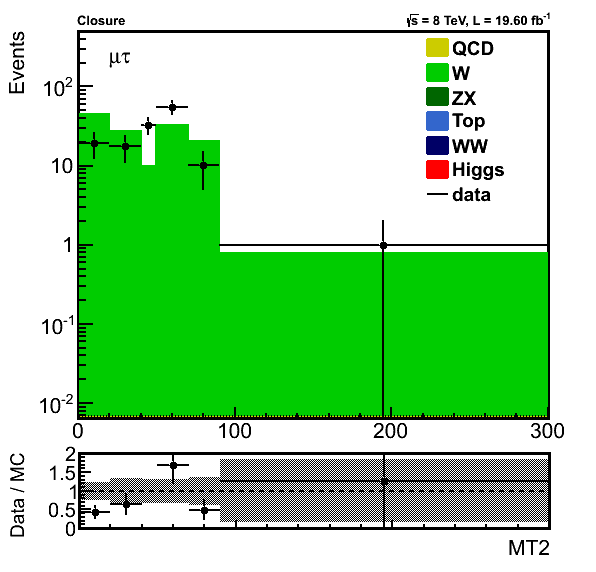
\includegraphics[width=0.475\textwidth,keepaspectratio=true]{FakeRateMuTau/Estimation_pfWJets_ExtraLepExcl_SameSignWeightedHiggs_tauMTApplied.png}
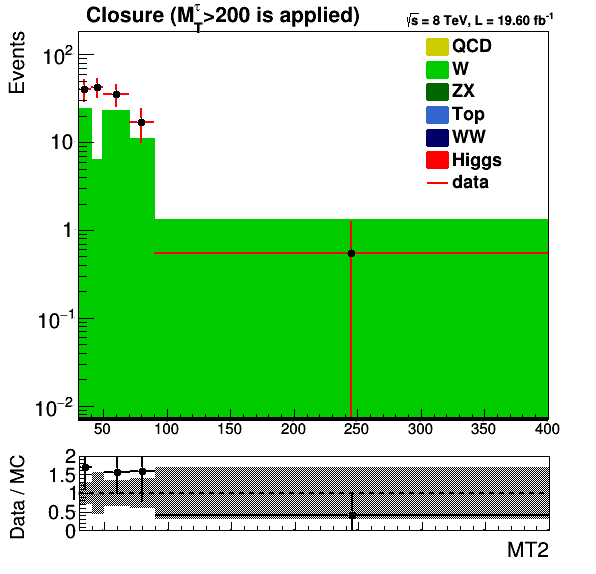
\includegraphics[width=0.475\textwidth,keepaspectratio=true]{FakeRateEleTau/closure_eletau_taumt200.png}
\caption{MC truth (green) compared to the result of the method in \muTau (left) and \eTau (right) channels. \wjets events with a fake \Tau are used for the closure.}
\label{fig:LepTauClusure}
\end{figure}
Figure \ref{fig:LepTauClusure} shows the results when the method is used to estimate the fake contamination of the \wjets events 
that pass the selection. 
The fake rate is evaluated in the same MC sample with similar procedure as the data, but  
also the MC truth are used to select the events with a fake \Tau and a prompt lepton. 
The measured fake rate is close to the value obtained in data and is 0.471 $\pm$  0.006. By comparing the fake rate in data and MC, 5\% relative systematic uncertainty is
assigned to the central values.
The method is applied on the same events with a loose \Tau selection and compared to the \wjets events with at least 
a fake \Tau. The requirement of prompt lepton is removed here.
%The fake rate measured in the same sign pairs is systematically less than the value 
%measured in the opposite sign pairs. The ratio is found to be 1.144 $\pm$ 0.019. The fake rate from data and \wjets are corrected by this ratio.
%As a cross check, the fake rate was measured in a different region when all cuts are same as signal selection, 
%except the cut on \MPT which is reversed to \MPT $<$ 30 \GeV. 
%The result is very close to $r_{\rm Fake}$ = 0.51 and the difference is taken as the systematic uncertainty
%of the fake rate (5\%).
%A similar value is measured for the fake rate. 
%For both fake rate and prompt rate, 5\% relative systematic uncertainty is assigned to the central values, although 
%by varying the selections, no significance change in the values is seen.
It can be seen that the estimation is close to the MC truth within the uncertainties.
The reported uncertainties for MC only contain the statistical uncertainties on the used numbers, but the estimations include 
the systematic uncertainties due to prompt and fake rate also. 
\begin{table}[!Hhtb]
\begin{center}
\caption{MC truth and estimation from the fake rate method in \muTau channel. \wjets events with a fake \Tau are used for the closure.}
\begin{tabular}{lccc}
\hline
\hline
   \mttwo range    &  \wjets& Estimation & ratio\\
\hline
\hline
40-50  & 9.91  $\pm$ 2.26 & 32.87 $\pm$ 8.45  & 3.32 $\pm$ 1.14 \\ 
50-70  & 32.53 $\pm$ 7.33 & 55.45 $\pm$ 11.72 & 1.70 $\pm$ 0.53 \\ 
70-90  & 20.45 $\pm$ 5.33 & 10.14 $\pm$ 5.17  & 0.49 $\pm$ 0.28\\
90-300 & 0.79  $\pm$ 0.47 &  0.99 $\pm$ 1.06  & 1.25 $\pm$ 1.53\\
\hline
\hline
\end{tabular}
\label{tbl:LepTauEstimationClosure}
\end{center}
\end{table}

\begin{table}[!Hhtb]
\begin{center}
\caption{MC truth and estimation from the fake rate method in \eTau channel. \wjets events with a fake \Tau are used for the closure.}
\begin{tabular}{lccc}
\hline
\hline
   \mttwo range    &  \wjets& Estimation & ratio\\
\hline
\hline
  40-50 &  6.34 $\pm$ 2.53 & 42.60 $\pm$ 10.80 & 6.72 $\pm$ 3.18 \\
  50-70 & 22.59 $\pm$ 5.43 & 35.43 $\pm$ 10.23 & 1.57 $\pm$ 0.59 \\
  70-90 & 10.91 $\pm$ 3.00 &  17.17 $\pm$ 7.45 & 1.57 $\pm$ 0.81 \\
 90-400 &  1.29 $\pm$ 0.62 &   0.54 $\pm$ 0.73 & 0.42 $\pm$ 0.60 \\
\hline
\hline
\end{tabular}
\label{tbl:EleTauEstimationClosure}
\end{center}
\end{table}
Table \ref{tbl:LepTauEstimationClosure} and \ref{tbl:EleTauEstimationClosure} compare the MC truth and the estimation of \wjets events 
from the method in different bins of \mttwo for \muTau and \eTau channels, respectively. 
Applying the method on data and comparing with MC truth is 
shown in figure \ref{fig:LepTauEstimationData}.
\begin{figure}[!Hhtb]
\centering
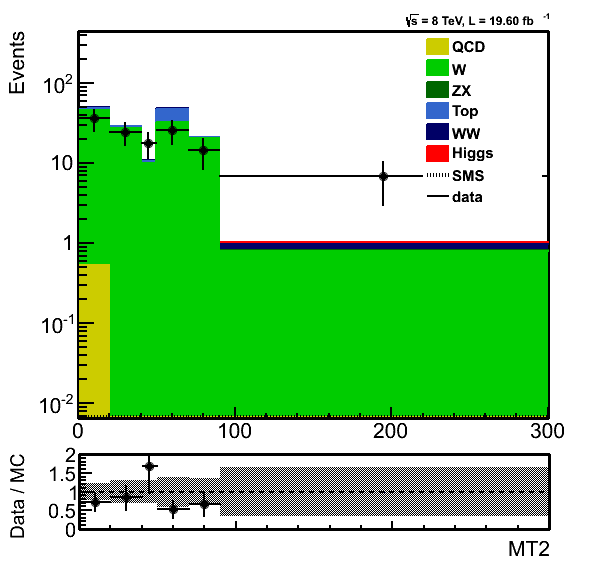
\includegraphics[width=0.45\textwidth,keepaspectratio=true]{FakeRateMuTau/Estimation_ExtraLepExcl_SameSignWeightedHiggs_tauMTApplied.png}
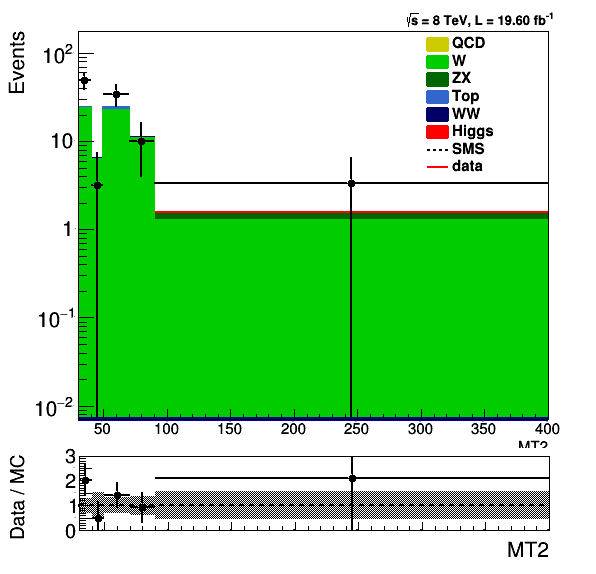
\includegraphics[width=0.45\textwidth,keepaspectratio=true]{FakeRateEleTau/estimation_eletau_taumt200.png}
\caption{Different MC events containing a fake \Tau are compared with the result of the method applied on data. The results for \muTau is shown in the left plot and \eTau is shown in the right plot.}
\label{fig:LepTauEstimationData}
\end{figure}
To select the MC events, all the selection cuts, except the \mttwo cut are applied. 
The MC truth are used to find the events with at least a fake \Tau. 
\begin{table}[!Hhtb]
\begin{center}
\caption{Numbers for figure \ref{fig:LepTauEstimationData} in \muTau channel.}
\begin{tabular}{lcccccccccc}
\hline
\hline
   \mttwo range &  QCD     &  ZX     &  W     & Top      & WW      & Higgs     & MC                 &  Estimation &ratio        &      \\   \hline
\hline
40-50  & 0 & 0.02 & 9.91  & 0.57  & 0.28 & 0.02  & 10.79 $\pm$ 2.30  & 21.55 $\pm$ 7.78  & 1.99 $\pm$ 0.84 \\
50-70  & 0 & 0.05 & 32.53 & 15.35 & 0.55 & 0.07  & 48.56 $\pm$ 13.77 & 31.18 $\pm$ 10.09 & 0.64 $\pm$ 0.28 \\ 
70-90  & 0 & 0    & 20.45 & 0.63  & 0.35 & 0.03  & 21.46 $\pm$ 5.37  & 17.39 $\pm$ 7.37  & 0.81 $\pm$ 0.39 \\
90-300 & 0 & 0.03 & 0.79  & 0     & 0.15 & 0.05  & 1.02  $\pm$ 0.48  & 8.15  $\pm$ 4.59  & 7.99 $\pm$ 5.86 \\

\hline
\hline
\end{tabular}
\label{tbl:LepTauEstimationData}
\end{center}
\end{table}

\begin{table}[!Hhtb]
\begin{center}
\caption{Numbers for figure \ref{fig:LepTauEstimationData} in \eTau channel.}
\begin{tabular}{lcccccccccc}
\hline
\hline
   \mttwo range &  QCD     &  ZX     &  W     & Top      & WW      & Higgs     & MC                 &  Estimation &ratio        \\   \hline
\hline
 40-50 & 0.00 & 0.00 &  6.34 & 0.00 & 0.11 & 0.02 &  6.48 $\pm$ 2.54 &  3.15 $\pm$ 4.47 & 0.48 $\pm$ 0.71 \\
 50-70 & 0.00 & 0.01 & 22.59 & 1.84 & 0.00 & 0.04 & 24.48 $\pm$ 5.56 & 34.53 $\pm$ 10.27 & 1.42 $\pm$ 0.53 \\
 70-90 & 0.00 & 0.01 & 10.91 & 0.00 & 0.06 & 0.02 & 11.00 $\pm$ 3.00 & 10.11 $\pm$ 6.16 & 0.92 $\pm$ 0.62 \\
90-300 & 0.00 & 0.19 &  1.29 & 0.00 & 0.02 & 0.07 &  1.57 $\pm$ 0.62 & 3.30  $\pm$ 3.35 & 2.12 $\pm$ 2.30 \\

\hline
\hline
\end{tabular}
\label{tbl:EleTauEstimationData}
\end{center}
\end{table}
Table \ref{tbl:LepTauEstimationData} and \ref{tbl:EleTauEstimationData} compare the MC truth and the estimation from the 
method in different bins of \mttwo for \muTau and \eTau channels, respectively. The numbers of the tightly selected events $T$ and 
non-tight events $NT$, used in equation \ref{eq:F} are 5(4) and 6(3) for \muTau(\eTau) in data.

The effect of varying the fake rate and prompt rate values within their statistical uncertainties has also been studied. 
It has been found in the order of a few percents which is negligible comparing to the statistical uncertainties due to lack of the statistics in the side bands.
The final values for fake \Tau contamination in different $\ell\Tau$ channels are summarized in table~\ref{Tab.FakeEstimation}. The statistical 
and systematical uncertainties are reported separately. Since the fake rate and  prompt rate are in common between the two 
$\ell\Tau$ channels, the total systematic uncertainties are considered fully correlated between the two channels.
\begin{table}[!Hhtb]
\begin{center}
\caption{The final estimation of the fake \Tau contribution in the signal region of the $\ell\Tau$ channels. The total systematic is the
quadratic sum of the fractional systematics. All uncertainties are relative.}
\begin{tabular}{lccccccccc}
\hline
\hline
Channel    & Total Fake & rel. Stat &  $f$ Sys & $p$ Sys & Total Sys \\\hline\hline
\muTau     &   8.15     &   56\%    &  18\%    & 5\%   & 59\%  \\
\eTau      &   3.30     &  101\%    &  17\%    & 2\%  & 102\%  \\
\hline
\hline
\end{tabular}
\label{Tab.FakeEstimation}
\end{center}
\end{table}
